\chapter{Theory of Classical Teletraffic}
\label{theory_of_classical_teletraffic}
\section{Telephone Traffic}
Traffic is a word originally used in the fields of transportation and trade to describe the volume of traffic and trade being transacted.
Teletraffic means traffic of communication.
The first type of teletraffic is a telephone.
There are two main definitions of traffic in telephony, one is simply the number of calls and the other is the duration of calls.
In some cases, the synergistic product of these two values is called traffic density, and this is referred to as traffic.\cite{teletraffic1954}

\section{Poisson Process}
A Poisson Process is a model for a series of discrete event where the average time between events is known, but the exact timing of events is random.
The arrival of an event is independent of the event before.\cite{poisson}
In terms of teletraffic, we know the amount of traffic in a unit of time, but we do not know at what interval it is communicated.

A Poisson Process meets the following criteria,\cite{poisson}
\begin{enumerate}
    \item Events are independent of each other. The occurrence of one event does not affect the probability another event will occur.
    \item The average rate (events per time period) is constant.
    \item Two events cannot occur at the same time.
\end{enumerate}

The Poisson process can explain the characteristics of telephone traffic mathematically well.
In particular, if we add an exponential distribution describing the time interval of events to the Poisson process, we can represent most of the actual telephone traffic.
In fact, the beginning of teletraffic theory was based on empirical studies and measurements, but with the observation of the Poisson nature of call arrivals, Poisson processes and exponential distributions became universal laws describing telephone traffic, and the curiosity of actually measuring it diminished.
This has allowed us to generate a steady stream of traffic, and many performance indicators can be accurately predicted. As a result, the telephone tends to be less blocked as a communication network.\cite{willinger1998mathematics}

\section{Acutual Traffic Pattern in IP Network}
With the advent of the Internet, Internet traffic appeared in the field of teletraffic as well.
Whereas telephone traffic is voice traffic, Internet traffic is data traffic.
Therefore, Internet traffic is the amount of packets/data moving across a computer network at any given time.

While telephones occupy a single communication channel for communication, the Internet divides data into packets for transmission, and packets of other communications also flow in the communication channel.
Therefore, the telephone is a centralized control system, while the Internet is a self-sustaining decentralized system. 
As a result, its overall behavior is very complex and difficult to understand.
Since the Internet is a self-sustaining distributed system, data that exceeds the transfer limit may suddenly be sent over the network.A sudden increase in the amount of data is called a burst.
One of the characteristics of Internet traffic is that, unlike telephone traffic, it cannot be explained by Poisson and exponential distributions.\cite{Fukuda2004}
This is because, as written earlier, the telephone and the Internet have different characteristics as communications.
  \begin{figure}[ht]
    \centering
    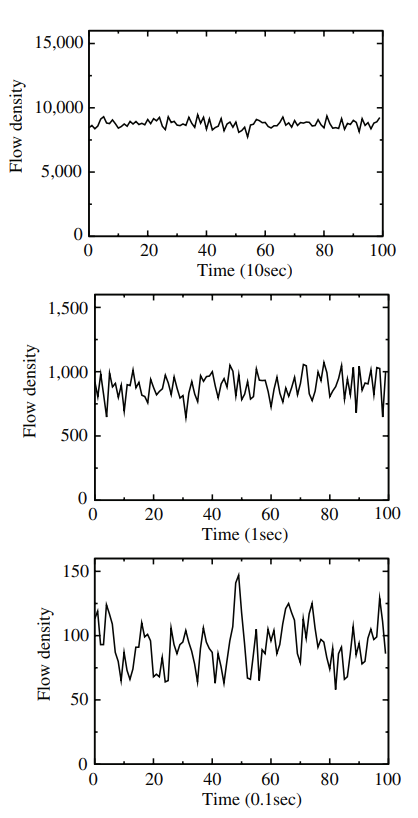
\includegraphics[width=5cm]{img/exponential.png}
    \caption{Exponential Traffic \protect \footnotemark}
    \label{fig:exponential}  
  \end{figure}
  \footnotetext{adapted from \cite{Fukuda2004} Fig.2}

Figure. \ref{fig:exponential} is shows a graph of exponential traffic by timescale.
As you can see, the exponential traffic is smoothed out as the timescale is increased.
\clearpage
  \begin{figure}[!ht]
    \centering
    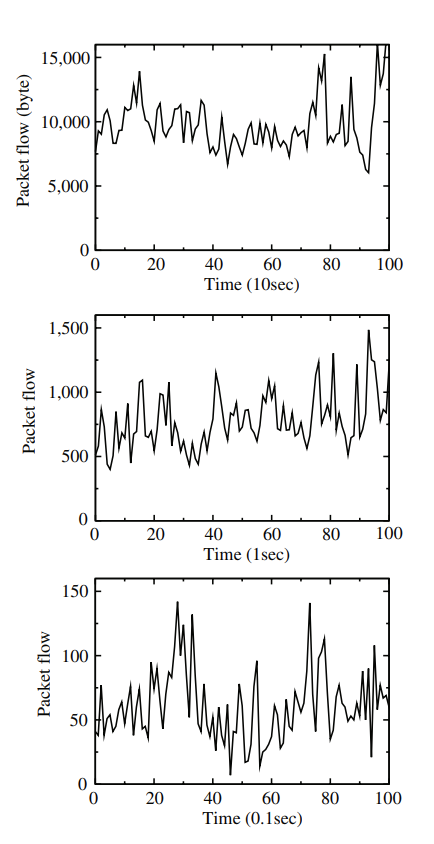
\includegraphics[width=5cm]{img/actual.png}
    \caption{Actual Traffic \protect \footnotemark}
    \label{fig:actual}  
  \end{figure}
  \footnotetext{adapted from \cite{Fukuda2004} Fig.2}

Figure. \ref{fig:actual} is shows a graph of actual traffic by timescale.
As you can see, even with a larger timescale, the actual traffic is bumpy.
This indicates that the traffic generation event occurrence is dependent on other events and that congestion can occur regardless of the timescale.

\section{Self-similar Model}

  \begin{figure}[ht]
    \centering
    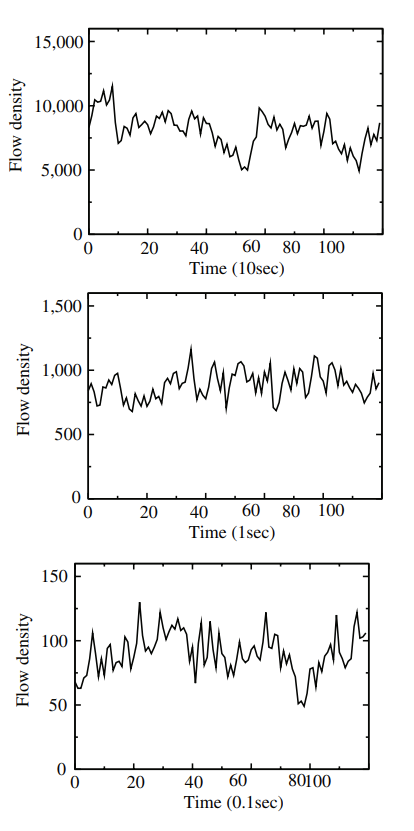
\includegraphics[width=5cm]{img/fractal.png}
    \caption{Self-Similar Traffic \protect \footnotemark}
    \label{fig:fractal}
  \end{figure}
  \footnotetext{adapted from \cite{Fukuda2004} Fig.2}
  \clearpage
  \begin{table}[ht]
    \centering
      \caption{The Features of Traffic \protect \footnotemark}
      \small
      \begin{tabular}{|c||l|l|}  \hline
         & Telephone & Internet \\ \hline \hline
        Link usage & Occupied, continuous & Shared, discrete \\ \hline
        Event occurrence & Poisson & Depends on other events \\ \hline
        Remarks & \begin{tabular}{l}Traffic can be expressed as Poisson, \\so traffic testing is easy. \end{tabular} & 
        \begin{tabular}{l}
        Events depends on other events \\ so traffic pattern is self-similar. \\ We can't use Poisson to test IP network.
        \end{tabular}\\ \hline
      \end{tabular}
  \end{table}
  \footnotetext{based on \cite{Ueda2007} Table.2}

\section{Traffic Matrix}
A Traffic Matrix is a matrix giving the traffic volumes between origin and destination in a network and has tremendously potential utility for IP network capacity planning and management.\cite{trafficmatrix}
\begin{figure}[!ht]
  \centering
  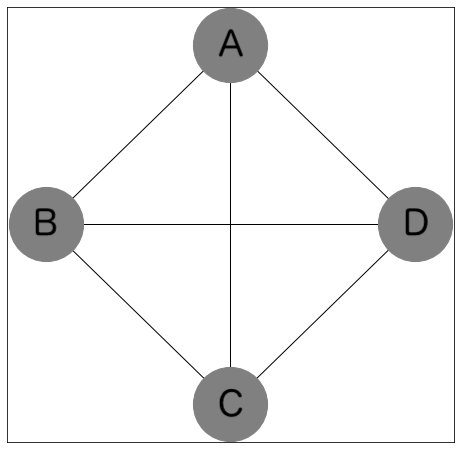
\includegraphics[width=5cm]{img/4node-graph.png}
  \caption{4-node Network}
  \label{fig:net} 
\end{figure}

\begin{screen}
  \begin{dfn}[Traffic Matrix]
    Consider a simple four-node, all-coupled network as shown in Fig.\ref{fig:net}.
    $T(i,j)$ means the amount of traffic from point j to point i. 
      \begin{equation}
          \begin{bmatrix}
            T(A,A) & T(A,B) & T(A,C) & T(A,D) \\
            T(B,A) & T(B,B) & T(B,C) & T(B,D) \\
            T(C,A) & T(C,B) & T(C,C) & T(C,D) \\
            T(D,A) & T(D,B) & T(D,C) & T(D,D) \\
          \end{bmatrix}
      \end{equation}
  \end{dfn}
\end{screen}


\section{Gravity Model}
Good for estimation and generation.
Talk about estimation and synthesization.

%%% Local Variables:
%%% mode: japanese-latex
%%% TeX-master: "./thesis"
%%% End:
